\documentclass{article}

\usepackage{fancyhdr}
\usepackage{extramarks}
\usepackage{amsmath}
\usepackage{amsthm}
\usepackage{amsfonts}
\usepackage{tikz}
\usepackage[plain]{algorithm}
\usepackage{algpseudocode}
\usepackage{enumerate}
\usepackage{graphicx}
\usepackage{pythonhighlight}
\usepackage{amssymb}
\usepackage{graphicx}
\usepackage{subfigure}

\usetikzlibrary{automata,positioning}

%
% Basic Document Settings
% 

\topmargin=-0.45in
\evensidemargin=0in
\oddsidemargin=0in
\textwidth=6.5in
\textheight=9.0in
\headsep=0.25in

\linespread{1.1}

\pagestyle{fancy}
\lhead{\hmwkAuthorName}
\chead{\hmwkClass\ (\hmwkClassInstructor): \hmwkTitle}
\rhead{\firstxmark}
\lfoot{\lastxmark}
\cfoot{\thepage}

\renewcommand\headrulewidth{0.4pt}
\renewcommand\footrulewidth{0.4pt}

\setlength\parindent{0pt}

%
% Create Problem Sections
%

\newcommand{\enterProblemHeader}[1]{
 \nobreak\extramarks{}{Problem \arabic{#1} continued on next page\ldots}\nobreak{}
 \nobreak\extramarks{Problem \arabic{#1} (continued)}{Problem \arabic{#1} continued on next page\ldots}\nobreak{}
}

\newcommand{\exitProblemHeader}[1]{
 \nobreak\extramarks{Problem \arabic{#1} (continued)}{Problem \arabic{#1} continued on next page\ldots}\nobreak{}
 \stepcounter{#1}
 \nobreak\extramarks{Problem \arabic{#1}}{}\nobreak{}
}

\setcounter{secnumdepth}{0}
\newcounter{partCounter}
\newcounter{homeworkProblemCounter}
\setcounter{homeworkProblemCounter}{1}
\nobreak\extramarks{Problem \arabic{homeworkProblemCounter}}{}\nobreak{}

%
% Homework Problem Environment
%
% This environment takes an optional argument. When given, it will adjust the
% problem counter. This is useful for when the problems given for your
% assignment aren't sequential. See the last 3 problems of this template for an
% example.
%
\newenvironment{homeworkProblem}[1][-1]{
 \ifnum#1>0
 \setcounter{homeworkProblemCounter}{#1}
 \fi
 \section{Problem \arabic{homeworkProblemCounter}}
 \setcounter{partCounter}{1}
 \enterProblemHeader{homeworkProblemCounter}
}{
 \exitProblemHeader{homeworkProblemCounter}
}

%
% Homework Details
% - Title
% - Due date
% - Class
% - Section/Time
% - Instructor
% - Author
%

\newcommand{\hmwkTitle}{Homework\ \#5}
\newcommand{\hmwkDueDate}{May 15, 2020}
\newcommand{\hmwkClass}{Reinforcement Learning}
\newcommand{\hmwkClassInstructor}{Professor Ziyu Shao}
\newcommand{\hmwkAuthorName}{Tianyuan Wu}
\newcommand{\hmwkAuthorID}{63305667}

%
% Title Page
%

\title{
 \vspace{2in}
 \textmd{\textbf{\hmwkClass:\ \hmwkTitle}}\\
 \normalsize\vspace{0.1in}\small{Due\ on\ \hmwkDueDate\ at 11:59am}\\
 \vspace{0.1in}\large{\textit{\hmwkClassInstructor}}
 \vspace{3in}
}

\author{\textbf{\hmwkAuthorName}\\ \hmwkAuthorID}
\date{}

\renewcommand{\part}[1]{\textbf{\large Part \Alph{partCounter}}\stepcounter{partCounter}\\}

%
% Various Helper Commands
%

% Useful for algorithms
\newcommand{\alg}[1]{\textsc{\bfseries \footnotesize #1}}

% For derivatives
\newcommand{\deriv}[1]{\frac{\mathrm{d}}{\mathrm{d}x} (#1)}

% For partial derivatives
\newcommand{\pderiv}[2]{\frac{\partial}{\partial #1} (#2)}

% Integral dx
\newcommand{\dx}{\mathrm{d}x}

% Alias for the Solution section header
\newcommand{\solution}{\textbf{\large Solution}}

% Probability commands: Expectation, Variance, Covariance, Bias
\newcommand{\E}{\mathrm{E}}
\newcommand{\Var}{\mathrm{Var}}
\newcommand{\Cov}{\mathrm{Cov}}
\newcommand{\Bias}{\mathrm{Bias}}

\begin{document}

\maketitle

\pagebreak

\begin{homeworkProblem} 
 \textbf{Solution}
 \begin{enumerate}
 \item [a)]
 First, we calculate the value function of $G$:
 \begin{equation}\nonumber\nonumber
 \begin{aligned}
 V(G) & = \sum_{t=0}^{\infty}(r_t \gamma^t)\\
 & = 1 + \gamma + \gamma^2 + \ldots \\
 & = \frac{1}{1-\gamma}
 \end{aligned}
 \end{equation}
 Then, we can observe that:
 $$V(s_{n-1}) = \frac{\gamma}{1-\gamma}$$
 $$V(s_{n-2}) = \frac{\gamma^2}{1-\gamma}$$
 $$\ldots$$
 $$V(s_1) = \frac{\gamma^{n-1}}{1-\gamma}$$
 \item [b)]
 Notice that when $\gamma > 0$, the value of $\gamma$ does not change the order of the value functions of states.
 That means, the optimal policy will not change: $\forall s_i, \pi(s_i) = a_1$. However, when $\gamma = 0$, 
 $\forall s_i, \pi(s_i) = a_1$ is also the optimal policy, but it's not the only optimal policy. 
 \item [c)]
 First, we still calculate the value funtions. For all $s_i$ we have:
 \begin{equation}\nonumber
 \begin{aligned}
 v_{\pi}^{new}(s_i) &= \sum_{t=0}^{\infty}(r_t \gamma^t)\\
 & = \sum_{t=0}^{\infty}((r_{old}+c)\gamma^t)\\
 & = v_{\pi}^{old}(s_i) + \frac{c}{1-\gamma}
 \end{aligned}
 \end{equation}
 Thus, the order of value functions of states will not change, and the 
 optimal policy will not changed.
 \item [d)]
 When changing $r_{new} = a(c+r_{old})$, the value functions will be:
 \begin{equation}\nonumber
 \begin{aligned}
 v_{\pi}^{new}(s_i) &= \sum_{t=0}^{\infty}(r_t \gamma^t)\\
 & = \sum_{t=0}^{\infty}(a(r_{old}+c)\gamma^t)\\
 & = a\cdot v_{\pi}^{old}(s_i) + \frac{ac}{1-\gamma}
 \end{aligned}
 \end{equation}
 So, if $a>0$, the order of $v(s_i)$ will not change, hence the optimal policy will not change.\\
 And if $a=0$, then all states will have $r(s_i)=0$ and any policy is the optimal policy, and the optimal
 value of all states is $0$.\\
 And if $a<0$, then any policy that never reaches to the goal state $G$ is the optimal policy, with value
 all states $v(s_i) = \frac{ac}{1-\gamma}$ and $v(G) = \frac{a(1+c)}{1-\gamma}$ for state $G$.
 \end{enumerate} 
\end{homeworkProblem}

\begin{homeworkProblem}
 \textbf{Solution}
 \begin{enumerate}
 \item [a)]
 The total discounted return is:
 $$V = \sum_{t=0}^{\infty}(r_t \gamma^t) = 0 + \gamma + \gamma^2 + \ldots = \frac{\gamma}{1-\gamma}$$
 \item [b)]
 The total discounted return is:
 $$V = \sum_{t=0}^{\infty}(r_t \gamma^t) = \frac{\gamma^2}{1-\gamma} + 0 +0 + \ldots = \frac{\gamma^2}{1-\gamma}$$
 Because $\gamma < 1$, the optimal action is $a_1$.
 \item [c)]
 For action $a_2$, notice that for all iterations, we have $V_n(s_2) = 0$, so we can observe that:
 $$Q(s_0, a_2) = \frac{\gamma^2}{1-\gamma}$$
 And for action $a_1$, the value iteration will update $Q(s_0, a_1)$ as:
 $$Q_{n+1}(s_0, a_1) = \gamma V_n(s_1) + 0$$
 $$V_{n+1}(s_0, a_1) = \gamma V_n(s_1) + 1$$
 Hence, we have:
 \begin{equation}\nonumber
 \begin{aligned}
 Q_{n+1}(s_0, a_1) &= 0 + \gamma (V_{n-1}(s_1) +1)\\
 &= \gamma (1 + \gamma + \gamma^2 + \ldots + \gamma^n V_0(s_1))\\
 &= \gamma (1 + \gamma + \gamma^2 + \ldots + \gamma^{n-1})\\
 &= \gamma \frac{1-\gamma^n}{1-\gamma}
 \end{aligned}
 \end{equation}
 And this value iteration will continues choose the sub-optimal action $a_2$ until 
 $Q(s_0, a_2) \le Q(s_0, a_1)$. So we set $Q_{n+1}(s_0, a_1) \le Q(s_0, a_2)$, and hence 
 we can solve $n^*$.\\
 By:
 $$\gamma \frac{1-\gamma^n}{1-\gamma} \le \frac{\gamma^2}{1-\gamma}$$
 we have:
 $$n^* \ge \frac{\log(1-\gamma)}{\log(\gamma)}$$
 Thus, the value iteration continues to choose the sub-optimal action until iteration $n^*$, 
 where $n^* \ge \frac{\log(1-\gamma)}{\log(\gamma)}$, the first inequality is proved.\\
 What's more,to prove the second inequality, we need the following lemma:\\
 $$\forall x \in (-1, 0], \log(1+x) \le \frac{2x}{2+x} $$
 which can be proved by move LHS and RHS together and taking the derivatives.\\
 Then we have: 
 \begin{equation}\nonumber
 \begin{aligned}
 \frac{\log(1-\gamma)}{\log(\gamma)} &= \frac{\log(1-\gamma)}{\log(1+\gamma-1)}\\
 & \ge \log(1-\gamma)\cdot \frac{1+\gamma}{2(\gamma-1)}\\
 &= \frac{1}{2}\cdot \frac{1+\gamma}{1-\gamma} \log\frac{1}{1-\gamma}\\
 & \ge \frac{1}{2} \log(\frac{1}{1-\gamma}) \frac{1}{1-\gamma}
 \end{aligned}
 \end{equation}
 \end{enumerate}
\end{homeworkProblem}


\begin{homeworkProblem}
 \textbf{Solution}
 \begin{enumerate}
 \item [a)]
 a)\\
 Notice that $\widetilde{Q}(s, \pi(s)) \ge \widetilde{Q}(s, \pi^*(s)$, so
 \begin{equation}\nonumber
 \begin{aligned}
 V^*(s)-Q^*(s,\pi(s)) &= V^*(s)-\widetilde{Q}(s,\pi(s))+\widetilde{Q}(s,\pi(s))-Q^*(s,\pi(s))\\ 
 & \le V^*(s) - \widetilde{Q}(s, \pi^*(s)) + \varepsilon\\
 &= Q^*(s, \pi^*(s)) - \widetilde{Q}(s, \pi^*(s)) + \varepsilon\\
 & \le 2\varepsilon
 \end{aligned}
 \end{equation}
 Thus we have: $V^*(s) - Q^*(s, \pi(s)) \le 2\varepsilon$
 \item [b)]
 \begin{equation}\nonumber
 \begin{aligned}
 V^*(s) - V_{\pi}(s) &= V^*(s) - Q^*(s, \pi(s)) + Q^*(s, \pi(s)) - V_{\pi}(s)\\
 & \le 2\varepsilon + Q^*(s, \pi(s)) - Q(s, \pi(s))\\
 & = 2\varepsilon + \gamma\mathbb{E}[V^*(s') - V_{\pi}(s')]
 \end{aligned}
 \end{equation}
 By the linearity of the expection, we have:
 \begin{equation}\nonumber
 \begin{aligned}
 V^*(s) - V_{\pi}(s) & \le 2\varepsilon + \gamma\mathbb{E}[V^*(s') - V_{\pi}(s')]\\
 & = 2\varepsilon (1 + \gamma + \gamma^2 \ldots )\\
 & = \frac{2\varepsilon}{1-\gamma}
 \end{aligned}
 \end{equation}
 Hence we have proved:
 $$V_{\pi}(s) \ge V^*(s) - \frac{2\varepsilon}{1-\gamma}$$
 \item [c)]
 \begin{equation}\nonumber
 \begin{aligned}
 Q(s_1, go) &= 2\varepsilon \lim_{t \to \infty} \sum_{t}(1 + \gamma + \gamma^2 + \ldots + \gamma^t)\\
 & = 2\varepsilon \frac{1}{1-\gamma}\\
 & = \frac{2\varepsilon}{1-\gamma}
 \end{aligned}
 \end{equation}
 \begin{equation}\nonumber
 \begin{aligned}
 Q(s_1, stay) &= 2\varepsilon \lim_{t \to \infty} \sum_{t}(0 + \gamma + \gamma^2 + \ldots + \gamma^t)\\
 & = 2\varepsilon \frac{\gamma}{1-\gamma}\\
 & = \frac{2\varepsilon\gamma}{1-\gamma} 
 \end{aligned}
 \end{equation}
 And the values are:
 \begin{equation}\nonumber
 \begin{aligned}
 & V^*(s_1) = \frac{2\varepsilon}{1-\gamma}\\
 & V^*(s_2) = \frac{2\varepsilon}{1-\gamma}
 \end{aligned}
 \end{equation}
 \item [d)]
 As observed, the difference between two state-value function is $2\epsilon$. Thus, we can simply build 
 a state-value function $\widetilde{Q}$ which makes $\pi(s_1) = stay$ the optimal action at $s_1$ (just set 
 $\widetilde{Q}(s_1, stay) = Q^*(s_1, stay) + \varepsilon$ and $\widetilde{Q}(s_1, go) = Q^*(s_1, go) - \varepsilon$),
 and then $V_{\pi}(s_1) - V^*(s_1) = -\frac{2\varepsilon}{1-\gamma}$. So there exists such an an approximate 
 state-action value function $\widetilde{Q}$, and the bound is tight.
 \end{enumerate}
\end{homeworkProblem}

\begin{homeworkProblem}
 \textbf{Solution}
 \begin{enumerate}
 \item [a)]
 \begin{equation}\nonumber
 \begin{aligned}
 v(s) &= \mathbb{E}[G_t|S_t=s]\\
 &= \mathbb{E}[R_{t+1} + \gamma R_{t+2} + \gamma^2 R_{t+3} + \ldots | S_t=s]\\
 &= \mathbb{E}[R_{t+1} + \gamma (R_{t+2} + \gamma R_{t+3} + \ldots) | S_t=s]\\
 &= \mathbb{E}[R_{t+1} + \gamma G_{t+1} | S_t=s]
 \end{aligned}
 \end{equation}
 Then we need to prove $\mathbb{E}[R_{t+1} + \gamma G_{t+1} | S_t=s] = \mathbb{E}[R_{t+1} + \gamma v(S_{t+1}) | S_t=s]$:\\
 First, we have 
 $$v(s) = \mathbb{E}[G_t|S_t=s], v(S_t) = \mathbb{E}[G_t|S_t], v(S_{t+1}) = \mathbb{E}[G_t|S_{t+1}]$$\\
 Second, by Adam's law, we have 
 $$\mathbb{E}[\mathbb{E}(Y|X,Z)|Z] = \mathbb{E}[Y|Z]$$.\\
 Let $Y=G_{t+1}, X=S_{t+1}$ and $Z=S_t$, we have:
 $$\mathbb{E}[\mathbb{E}(G_{t+1}|S_{t+1},S_t)|S_t] = \mathbb{E}[G_{t+1}|S_t] = \mathbb{E}[\mathbb{E}[G_{t+1}|S_{t+1}]|S_t]$$
 So,$$\mathbb{E}[\mathbb{E}(G_{t+1}|S_{t+1},S_t)|S_t] = \mathbb{E}[v(S_{t+1})|S_t]$$.\\
 Thus, $$\mathbb{E}[G_{t+1}|S_t=s] = \mathbb{E}[v(S_{t+1})|S_t]$$.\\
 Then, we can observe that:
 \begin{equation}\nonumber
 \begin{aligned}
 v(s) &= \mathbb{E}[G_t | S_t = s]\\
 &= \mathbb{E}[R_{t+1} + \gamma G_{t+1} |S_t = s]\\
 &= \mathbb{E}[R_{t+1}|S_t=s] + \gamma \mathbb{E}[G_{t+1} |S_t = s]\\
 &= \mathbb{E}[R_{t+1}|S_t=s] + \gamma \mathbb{E}[v(S_{t+1}) |S_t = s]\\
 &= \mathbb{E}[R_{t+1} + \gamma v(S_{t+1}) |S_t = s]
 \end{aligned}
 \end{equation}
 Now, we've proved $v(s) = \mathbb{E}[R_{t+1} + \gamma v(S_{t+1}) |S_t = s]$.\\
 Then, we have:
 \begin{equation}\nonumber
 \begin{aligned}
 v(s) &= \mathbb{E}[R_{t+1} + \gamma v(S_{t+1}) |S_t = s]\\
 &= R_s + \gamma \sum_{s' \in S}{\mathbb{E}[v(S_{t+1}|S_t=s, S_{t+1}=s')]P(S_{t+1}=s' | S_t=s)}\\
 &= R_s + \gamma \sum_{s' \in S}{v(s')P_{ss'}}
 \end{aligned}
 \end{equation}
 Hence, we've proved the Bellman equation of MRP.
 \item [b)]
 First, we know: 
 $$q_{\pi}(s,a) = \mathbb{E}_{\pi}[G_t | S_t=s, A_t=a]$$
 $$q_{\pi}(S_t,A_t) = \mathbb{E}_{\pi}[G_t |S_t, A_t]$$
 $$q_{\pi}(S_t,A_{t+1}) = \mathbb{E}_{\pi}[G_{t+1} |S_{t+1}, A_{t+1}]$$
 Then we use Adam's law with extra conditioning,
 Let $Y=G_{t+1}$, $Z=(S_t, A_t)$ and $X=(S_{t+1}, A_{t+1})$
 then we have:
 \begin{equation}\nonumber
 \begin{aligned}
 \mathbb{E}[G_{t+1}|S_t, A_t] &= \mathbb{E}[\mathbb{E}[G_{t+1}|S_{t+1}, A_{t+1}, S_t, A_t]|S_t, A_t]\\
 &= \mathbb{E}[\mathbb{E}[G_{t+1}|S_{t+1}, A_{t+1}]|S_t, A_t]
 &= \mathbb{E}[q_{\pi}(S_{t+1}, A_{t+1})|S_t, A_t]
 \end{aligned}
 \end{equation}
 So, $\mathbb{E}_{\pi}[G_{t+1}|S_t=s, A_t=a] = \mathbb{E}_{\pi}[q_{\pi}(S_{t+1}, A_{t+1})|S_t=s, A_t=a]$\\
 Then we have:
 \begin{equation}\nonumber
 \begin{aligned}
 q_{\pi}(s,a) &= \mathbb{E}_{\pi}[G_{t}|S_t=s, A_t=a]\\
 &= \mathbb{E}_{\pi}[R_{t+1}+\gamma G_{t+1}|S_t=s, A_t=a]\\
 &= \mathbb{E}_{\pi}[R_{t+1}|S_t=s, A_t=a] +\gamma \mathbb{E}_{\pi}[G_{t+1}|S_t=s, A_t=a]\\
 &= \mathbb{E}_{\pi}[R_{t+1}+\gamma q_{\pi}(S_{t+1}, A_{t+1})|S_t=s, A_t=a]
 \end{aligned}
 \end{equation}
 Then for $Q^{\pi}$, we have:
 \begin{equation}\nonumber
 \begin{aligned}
 & \mathbb{E}_{\pi}[q_{\pi}(S_{t+1}, A_{t+1})|S_{t+1}=s', S_t=s, A_t=a] \\
 &= \mathbb{E}_{\pi}[q_{\pi}(S_{t+1}, A_{t+1})|S_{t+1}=s']\\
 &= \sum_{a \in A} \mathbb{E}_{\pi}[q_{\pi}(S_{t+1}, A_{t+1})|S_{t+1}=s', A_{t+1}=a] P( A_{t+1}=a | S_{t+1}=s')\\
 &= \sum_{a \in A} a_{\pi}(s',a)\pi(a|s')\\
 &= v^{\pi}(s')
 \end{aligned}
 \end{equation}
 Then we have:
 \begin{equation}\nonumber
 \begin{aligned}
 & \mathbb{E}_{\pi}[q_{\pi}(S_{t+1}, A_{t+1})| S_t=s, A_t=a]\\
 &= \sum_{s' \in S} \mathbb{E}_{\pi}[q_{\pi}(S_{t+1}, A_{t+1})|S_{t+1}=s', A_t=a, S_t=s] P( A_{t+1}=a | S_{t}=s, A_t=a)\\
 &= \sum_{s' \in S} v_{\pi}(s')P_{ss'}^{a}
 \end{aligned}
 \end{equation}
 Thus, 
 \begin{equation}\nonumber
 \begin{aligned}
 q_{\pi}(s,a) &= \mathbb{E}_{\pi}[R_{t+1}+\gamma q_{\pi}(S_{t+1}, A_{t+1})|S_t=s, A_t=a]\\
 &= \mathbb{E}_{\pi}[R_{t+1}|S_t=s, A_t=a] + \gamma \mathbb{E}_{\pi}[q_{\pi}(S_{t+1}, A_{t+1})|S_t=s, A_t=a]\\
 &= R_{s}^{a} + \gamma \sum_{s' \in S}v_{\pi}(s')P_{ss'}^{a}
 \end{aligned}
 \end{equation}
 And for $v_{\pi}$, we have
 $$v_{\pi}(s) = \sum_{a \in A} \pi(a|s) (R_{s}^{a} + \gamma \sum_{s' \in S}v_{\pi}(s')P_{ss'}^{a})$$
 and for $q_{\pi}(s)$, we have
 $$q_{\pi}(s,a) = R_{s}^{a} + \gamma \sum_{s' \in S}P_{ss'}^{a}(\sum_{a' \in A}(\pi(a'|s')q_{\pi}(s',a')))$$
 Now, we've proved the Bellman equation of expection of MDP.
 \item [c)]
 For $Q^*$, first we know:
 $$q_{\pi}(s,a) = R_s ^a + \gamma \sum_{s' \in S} v_{\pi}(s')P_{ss'}^{a}$$
 and 
 $$q_{*}(s,a) = \max_{\pi}(q_{\pi}(s,a)) = R_s ^a +\gamma \sum_{s' \in S} \max_{\pi}(v_{\pi}(s'))P_{ss'}^{a} =R_s ^a + \gamma \sum_{s' \in S} v^{*}_{\pi}(s')P_{ss'}^{a}$$
 Then, for 
 $$\mathbb{E}(R_{t+1}|S_t=s, A_t=a) = R_s^a$$
 and
 \begin{equation}\nonumber
 \begin{aligned}
 & \mathbb{E}[v_* (S_{t+1})|S_t=s, A_t=a] \\
 &= \sum_{s' \in S} \mathbb{E}[v_* (S_{t+1}) |S_{t+1} = s', S_t = s, A_t = a]\cdot P(S_{t+1} = s'| S_t = s, A_t = a)\\
 &= \sum_{s' \in S} v_*(s') P_{ss'}^a
 \end{aligned}
 \end{equation}
 Then we have:
 $q_*(s,a) = \mathbb{E}[R_{t+1} + \gamma v_* (S_{t+1})|S_t, A_t]$
 for $v_{*}(s) = \max_{a}(q_*(s,a))$, we know:
 $$v_{*}(s) = \max_{a}\mathbb{E}[R_{t+1} + \gamma v_* (S_{t+1})|S_t=s, A_t=a]$$
 So, we've proved the Bellman Optimality Equations for Markov Decision Processes (MDPs)
 $$v_{*}(s) = \max_{a}(R_s ^a + \gamma \sum_{s' \in S} v^{*}_{\pi}(s')P_{ss'}^{a})$$
 $$q_{*}(s,a) = R_s ^a + \gamma \sum_{s' \in S} v^{*}_{\pi}(s')P_{ss'}^{a}$$
 \end{enumerate}
\end{homeworkProblem}

\begin{homeworkProblem}
 \textbf{Solution}
 \begin{enumerate}
 \item [a)] 
 We use the matrix form of MRP, Here we have:
 $$v = R + \gamma Pv$$
 so
 $$v = (I-\gamma P)^{-1}R$$
 Let
 $$R = \begin{bmatrix}
 -2 \\ -2 \\ -2 \\ 10 \\ 1 \\ -1 \\ 0
 \end{bmatrix}$$
 and $P$ be the transition matrix (7*7) of the student MDP
 we can solve the $v$:
 $$v = \begin{bmatrix}
 -12.53 \\ 1.46 \\ 4.32 \\ 10.00 \\ 0.80 \\ -22.54 \\ 0
 \end{bmatrix}$$
 So, the states values are:\\
 $$v(Sleep) = 0$$
 $$v(C_3) = 4.3$$
 $$v(Pass) = 10.0$$
 $$v(C_2) = 1.5$$
 $$v(C_1) = -13$$
 $$v(Pub) = 0.8$$
 $$v(FB) = -23$$ 
 \item [b)]
 we know that
 $$v_{\pi}(s) = \sum_{a \in A}\pi(a|s)[R_s^a + \gamma \sum_{s' \in S} P_{ss'}^a v_{\pi}(s)]$$
 Let's define $v_j = v_{\pi}(s_j)$, and we have:
 $$v_1 = v_{\pi}(s_1) = 0.5*(R_{s_1}^{study} + v_{\pi}(s_2)) + 0.5*(R_{s_1}^{FB} + v_{\pi}(s_4)$$
 $$= 0.5(-2 + v_2) + 0.5(-1 + v_4)$$
 similarly,
 $$v_2 = v_{\pi}(s_2) = 0.5*(-2 + v_3) + 0.5*(0+0)$$
 $$v_3 = v_{\pi}(s_3) = 0.5*(1+0.2v_1+0.4v_2 + 0.4v_3) + 0.5(10+0)$$
 $$v_4 = v_{\pi}(s_4) = 0.5*(0+v_1) + 0.5*(-1+v_4)$$
 Hence, we can observe:
 $$v_1 = -1.3, v_2 = 2.7, v_3 = 7.4, v_4 = -2.3$$
 So, we can get the state-action value:
 $$q_{\pi}(s_1, study) = -2 + 1v_2 = -2 + 2.7 = 0.7$$
 $$q_{\pi}(s_1, FB) = -1 +1v_4 = -1-2.3= -3.3$$
 $$q_{\pi}(s_2, sleep)=0+0=0$$
 $$q_{\pi}(s_2, study) = -2+1v_3 = -2+7.4=5.4$$
 $$q_{\pi}(s_3, study) = 10 + 0 = 10$$
 $$q_{\pi}(s_3, pub) = 1 + 0.2v_1 + 0.4v_2 + 0.4v_3 = 4.78$$
 $$q_{\pi}(s_4, FB) = -1 + v_4 = -1-2.3=-3.3$$
 $$q_{\pi}(s_4, Quit) = 0 + v_1 = 0-1.3=-1.3$$
 \item [c)]
 We know that 
 $$q_{\pi}(s,a) = R_s ^a + \gamma \sum_{s' \in S'}(P_{ss'}^a v_{\pi}(s'))$$
 $$q_{*}(s,a) = \max_{\pi}(q_{\pi}(s,a))$$
 Since $v_{\pi}(sleep) = 0$, then we have 
 $$\forall \pi, q_{\pi}(s_2, sleep) = R_{s_2}^{sleep} + 1\cdot v_{\pi}(sleep) = 0+0=0$$
 so $q_{*}(s_2, sleep) =0$.\\
 On the other hand, 
 $$\forall \pi, q_{\pi}(s_3, study) = 10+0 = 10$$
 so, $q_{*}(s_2, study) =10$.\\
 Then,
 $$q_{*}(s_1, study) = R_{s_1}^{study} + \gamma P_{s1,s2}^{study}\max_{a'} q_{*}(s_2, a') = -2 + \max(0, q_*(s_2, study))$$
 $$q_{*}(s_1,FB) = -1 + \max(q_*(s_4, FB), q_*(s_4, quit))$$
 $$q_*(s_2, sleep) = 0$$
 $$q_*(s_2, study) = -2 + \max(10, q_*(s_3, pub))$$
 $$q_*(s_3, study) = 10$$
 $$q_*(s_3, pub) = 1 + 0.2\max(q_*(s_1, study), q_*(s_1, FB)) + 0.4\max(q_*(s_2, study), 0) + 0.4\max(q_*(s_3, pub),10)$$
 $$q_*(s_4, FB) = -1 + \max(q_*(s_4, FB), q_*(s_4, Quit))$$
 $$q_*(s_4, Quit) = 0 + \max(q_*(s_1, Study), q_*(s_1, FB))$$
 we can observe that
 $$q_*(s_2, study) = -2 + \max(10, q_*(s_3, pub)) \ge 8$$
 $$q_{*}(s_1, study) = -2 + \max(0, q_*(s_2, study)) \ge 6$$
 and 
 $$q_*(s_4, FB) < q_*(s_4, Quit)$$
 $$q_*(s_1, FB) = -1 + q_*(s_4, Quit)$$
 $$q_*(s_4, Quit) = -2 + q_*(s_2, study)$$
 $$q_*(s_3, pub) = 0.6 + 0.6q_8(s_2, study) + 4$$
 Hence, we can solve the optimal state-action values:
 $$q_*(s_1, study)= -2+8=6$$
 $$q_*(s_3, pub) = 4.6+0.6*8=9.4$$
 $$q_*(s_4, Quit) = 6$$
 $$q_*(s_4, FB) = -1+6=5$$
 $$q_*(s_1, FB) = -1+6= 5$$
 and optimal state values:
 $$v_*(s_1) = \max_{a}(q_*(s_1, study), q_*(s_1, FB)) = \max(5,6)=6$$
 $$v_*(s_2) = \max_{a}(q_*(s_2, study), q_*(s_2, sleep)) = \max(8,0)=8$$
 $$v_*(s_3) = \max_{a}(q_*(s_3, study), q_*(s_3, pub)) = \max(10,9.4)=10$$
 $$v_*(s_4) = \max_{a}(q_*(s_4, Quit), q_*(s_4, FB)) = \max(6,5)=6$$
 $$v_*(sleep)=10$$
 and the optimal policy is:
 $$s_1: study$$
 $$s_2: study$$
 $$s_3: study$$
 $$s_1: Quit$$
 $$sleep: sleep$$
 \end{enumerate}
\end{homeworkProblem}


\begin{homeworkProblem}
 \textbf{Solution}
 \begin{enumerate}
 \item [a)]
 The implementation is in the ".ipynb" file, and the result is ($\gamma=0.9$, and round to 1 decimal digits):
 \begin{figure}[h]
 \begin{center}
 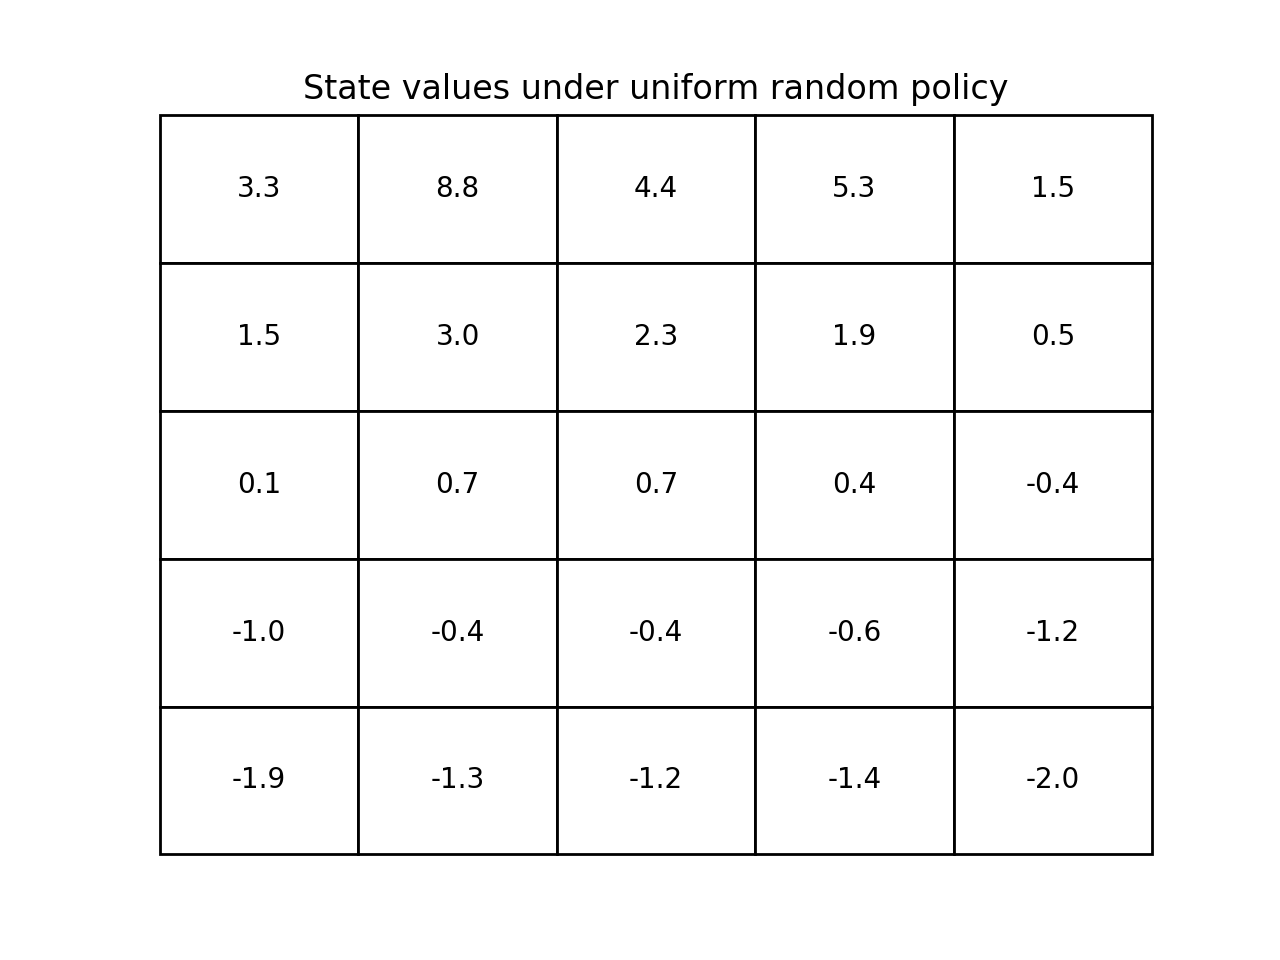
\includegraphics[scale=0.4]{sv.png}
 \caption{State values}
 \end{center}
 \end{figure}
 \item [b)]
 The implementation is in the ".ipynb" file, and the result is ($\gamma=0.9$, and round to 1 decimal digits)\\
 
 First, we calculate the state-action values of go up, down, left and right.
 \begin{figure}[H]
 \begin{center}
 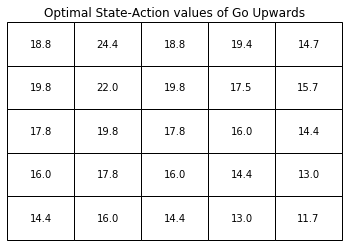
\includegraphics[scale=0.4]{osavu.png}
 \end{center}
 \caption{Optimal state-action values of Go up}
 \end{figure}
 \begin{figure}[H]
 \begin{center}
 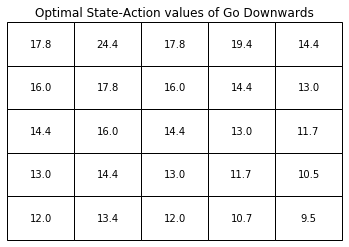
\includegraphics[scale=0.4]{osavd.png}
 \end{center}
 \caption{Optimal state-action values of Go Down}
 \end{figure}
 \begin{figure}[H]
 \begin{center}
 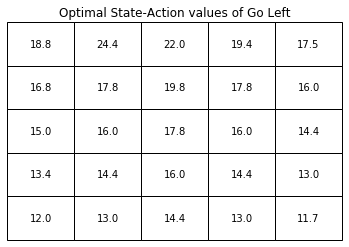
\includegraphics[scale=0.4]{osaul.png}
 \end{center}
 \caption{Optimal state-action values of Go Left}
 \end{figure}
 \begin{figure}[H]
 \begin{center}
 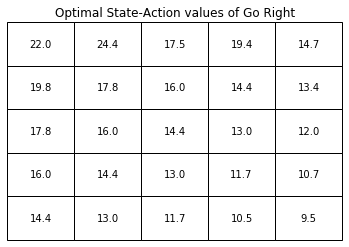
\includegraphics[scale=0.4]{osaur.png}
 \end{center}
 \caption{Optimal state-action values of Go Right}
 \end{figure}

 Then, take the $\max$ of them, and get the optimal state values.
 \begin{figure}[H]
 \begin{center}
 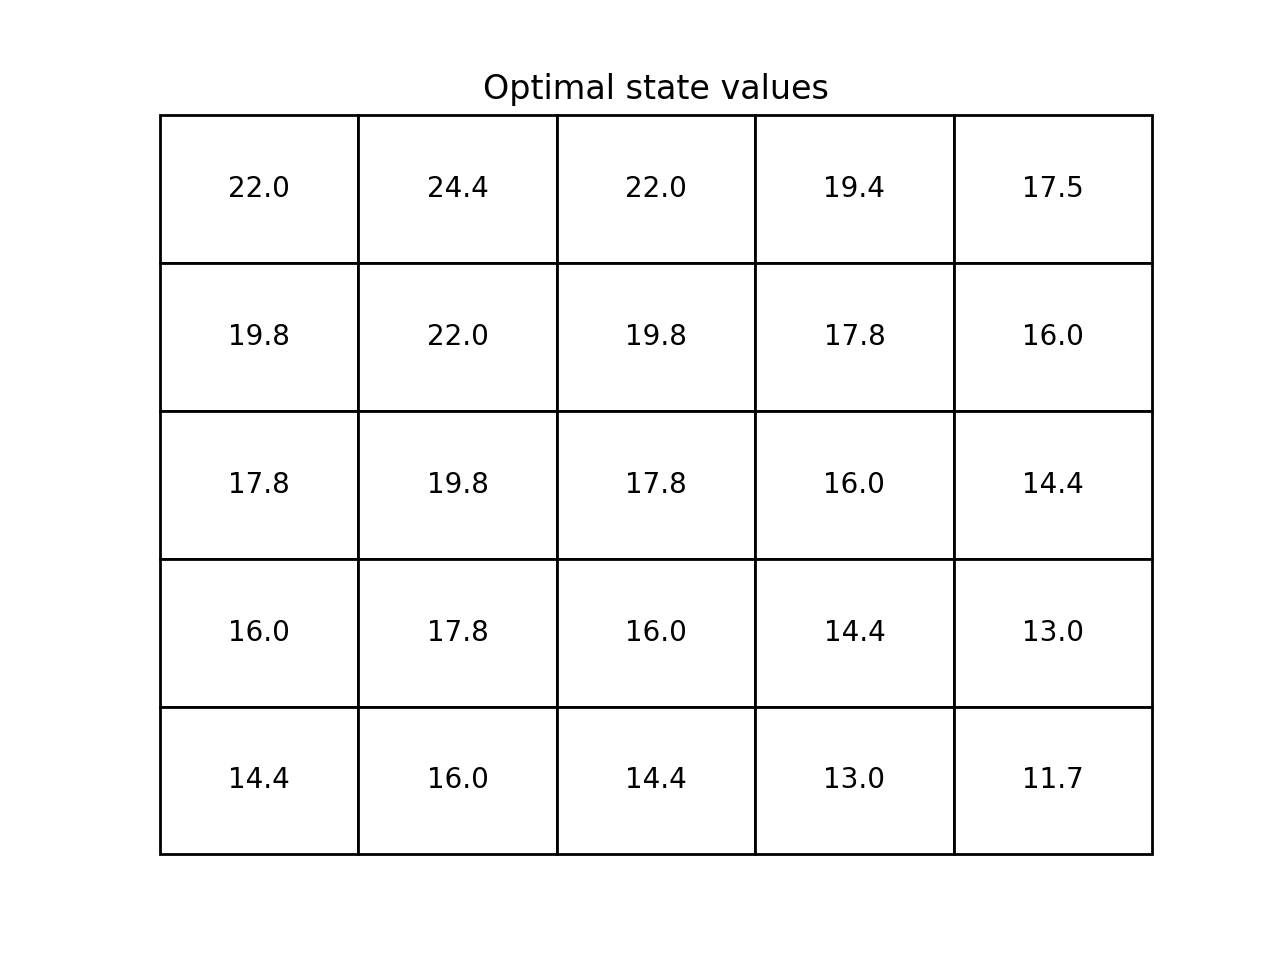
\includegraphics[scale=0.4]{osv.png}
 \end{center}
 \caption{Optimal state values}
 \end{figure}
 \pagebreak
 And finally, get the optimal policy.
 \begin{figure}[H]
 \begin{center}
 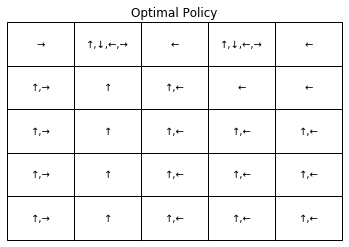
\includegraphics[scale=0.4]{op.png}
 \end{center}
 \caption{Optimal Policy}
 \end{figure}
 \end{enumerate}
\end{homeworkProblem}


\begin{homeworkProblem}
 \textbf{Bonus1 - Solution}\\
 Let $V_n(x)$ denote the maximal expected return if the gambler has a
 present fortune of $x$ and is allowed $n$ more gambles. Let $\alpha$ 
 be the fraction of fortune that he bets in the following action. (e.g. 
 $\alpha=0.5$ means he use $0.5x$ to bet in the following action). Then 
 we have the Bellman optimal equation:
 $$V_{n}(x) = \max_{0 \le \alpha \le 1} (p\cdot V_{n-1}((1+\alpha)x) + q\cdot (V_{n-1}((1-\alpha)x))$$
 and the boundary condition is:
 $$V_{0} = \log x$$
 So, we have:
 $$V_{1}(x) = \max_{0 \le \alpha \le 1} (p\log (x+\alpha x) + q\log (x- \alpha x)) \\= \max_{0 \le \alpha \le 1}((p\log (1+\alpha) + q\log (1- \alpha))) + \log x$$
 Now we only need to consider the following part, let:
 $$f(\alpha) = p\log (1+\alpha) + q\log (1- \alpha)$$
 Take derivatives to 0:
 $$\frac{df(\alpha)}{d\alpha} = \frac{p}{1+\alpha} - \frac{q}{1-\alpha} = 0$$
 and use $p +q=1$, we have:
 $$\alpha = p-q$$
 Also, the second-order derivative at $\alpha=p-q$ is less than 0, so it's the maximium point of $f(\alpha)$.\\
 So, when $p \le q$ (i.e. $p \le \frac{1}{2}$), the maximium point in $\alpha \in [0,1]$ is $\alpha=0$. And we 
 can do it recursively and observe that in this case, $V_{n}(x) = logx$, and the optimal policy under $p \le \frac{1}{2}$ 
 is \textbf{Always bet 0}. \\
 Now consider the case that $p > q$ (i.e. $p > \frac{1}{2}$), now the maximium point is $\alpha = p-q$, and the maximium 
 value is 
 $$f_{max}(\alpha) = \log 2 + p \log p + q \log q$$
 So we have:
 $$V_{1}^*(x) = \log 2 + p \log p + q \log q + \log x$$
 And we can get $V_{2}(x)$:
 $$V_2(x) = \max_{0 \le \alpha \le 1} (p\log (x+\alpha x) + q\log (x- \alpha x)) + \log 2 + p \log p + q \log q$$
 We also take the derivatives by a similarly way, and we can observe:
 $$V_{2}^*(x) = 2(\log 2 + p \log p + q \log q) + \log x$$
 Hence, we can do it recursively and get:
 $$V_{n}^*(x) = n(\log 2 + p \log p + q \log q) + \log x$$
 And the optimal policy is under this situation ($p > \frac{1}{2}$) is:\\
 \textbf{Always to bet the fraction} $p - q$ \textbf{of one's present fortune.}
\end{homeworkProblem}

\begin{homeworkProblem}
 \textbf{Bonus2 - Solution}\\
 In this problem, We say we're at $state_i$ if the $i^{th}$ offer has just been presented
 and it is the best of the $i$ offers already presented. Letting $V(i)$ denote
 the best we can do in this position, we know that $V$ satisfies:
 $$V_{i} = \max\{P(i), H(i)\}$$
 Where $P(i)$ denotes \textbf{the best offer is choosen if we accept the $i^{th}$ offer}, 
 and $H(i)$ denotes \textbf{the best we can do if we reject the $i^{th}$ offer}.\\
 Now we have that:
 \begin{equation}\nonumber
 \begin{aligned}
 P(i) &= P(\text{offer is best of n} | \text{offer is best of first i}) \\
 &= \frac{1/n}{1/i} = \frac{i}{n}
 \end{aligned}
 \end{equation}
 Hence, 
 $$V(i) = \max \{\frac{i}{n}, H(i)\}, \quad i = 1, 2, \ldots, n$$
 So, we know that $H(i)$ is the maximal probability of accepting
 the best offer when we have rejected the first $i$ offers. It's obviously 
 that when $i$ is increasing, $\frac{i}{n}$ increases, while $H(i)$ decreases.
 So, there exists some number $j$ which satisfies:
 $$\frac{i}{n} \le H(i), \quad i \le j$$
 $$\frac{i}{n} > H(i),\quad i > j$$
 Hence, the optimal policy is: for some $j$( $j < n — 1$), reject the first $j$ offers 
 and then accept the first offer which satisfies it has higher value than any of its predecessors. \\
 Now let $P_{j}(best)$ be the probability of get the best offer under this policy, so we have that:
 $$P_{j}(best) = \sum_{i=1}^{n-j}(P_j(best|(j+i) \text{is accepted}) \cdot P((j+i) \text{is accepted}))$$
 and we know:
 $$P_j(best|(j+i) \text{is accepted}) = \frac{i+j}{n}$$
 and:
 \begin{equation}\nonumber
 \begin{aligned}
 & P((j+i) \text{is accepted}) \\
 &= P(\text{best of first j offers = best of first (i+j) offers}, (i+j)^{th} \text{is the best of $i+j$ offers} )\\
 &= (\frac{j}{i+j-1})(\frac{1}{i+j})
 \end{aligned}
 \end{equation}
 Thus we can calculate the $P_j(best)$:
 \begin{equation}\nonumber
 \begin{aligned}
 P_j(best) &= \frac{j}{n}\sum_{i=1}^{n-j}(\frac{1}{i+j-1})\\
 &= \frac{j}{n}\sum_{k=j}^{n-1}\frac{1}{k}\\
 &\approx \frac{j}{n} \int_{j}^{n-1} (\frac{1}{x})dx\\
 &= \frac{j}{n} \log (\frac{n-1}{j}) \approx \frac{j}{n} \log (\frac{n}{j})
 \end{aligned}
 \end{equation}
 Now we let 
 $$f(x) = \frac{x}{n} \log (\frac{n}{x}) $$
 Take the derivatives to 0, we have:
 $$\frac{df(x)}{dx} = \frac{1}{n} \log(\frac{n}{x}) - \frac{1}{n} = 0$$
 and we can solve that:
 $$x = \frac{n}{e}$$
 Also, the second-order derivative is less than 0 at $x= \frac{n}{e}$, so, it's the maximium point.
 Then we have:
 $$f(\frac{n}{e}) = \frac{1}{e}$$
 So, the optimal policy is: when $n$ is large, approximately to let the
 fraction $\frac{1}{e}$ of all offers be rejected and then accept the first candidate. The
 probability that this procedure will result in the best offer is roughly $\frac{1}{e}$.
\end{homeworkProblem}

\begin{homeworkProblem}
    \textbf{Bonus3 - Solution}
    \begin{enumerate}
    \item [a)]
        This is not the optimal solution for it's myopic, which only concentrates on the 
        short-term rewards, regardless of long-term rewards. The counter example is, assume that 
        $\frac{\alpha_1}{\alpha_1 + \beta_1} = \frac{\alpha_2}{\alpha_2 + \beta_2}$. 
        The suggested index rule is the same between the two arms, though if, 
        for example, $\alpha_2 + \beta_2 >> \alpha_1 + \beta_1$, so the variance of $\theta_1$ is 
        much greater than that of $\theta_2$, it is much more likely that further pulls on arm
        1 will lead to appreciable changes in than it is for comparable changes to occur when 
        arm 2 is pulled. This strongly suggests that it must be better to pull arm 1, as 
        the expected immediate rewards are the same in both cases, and there is more information 
        to be gained by pulling arm 1; information which may be used to achieve higher expected 
        rewards later on. 
    \item [b)]
        If arm1 is pulled, the probability of a success is the expectation of $\theta_1$: 
        $$\hat{\theta}_1 = \mathbb{E}[Beta(\alpha_1, \beta_1)] = \frac{\alpha_1}{\alpha_1+ \beta_1}$$
        This quantity is the multiplier of the first expression of $R_1$, 
        which is the expected total reward under an optimal policy after the first pull, 
        conditional on this resulting in asuccess. To see this, note that the success yields an immediate 
        reward of 1and results, by Bayes’ theorem, in a posterior distribution $Beta(\alpha_1, \beta_1 +1)$. 
        The prior distribution for $\theta_2$ remains the current distribution, as a pull on arm1 yields no 
        effects on $\theta_2$. Thus the expected total reward under an optimal policy from this point onwards is 
        exactly the same as the expected total reward from the outset with priors which are $Beta(\alpha_1+1,\beta_1)$
        and $Beta(\alpha_2,\beta_2)$, except for an additional factor $\gamma$, namely $\gamma R(\alpha_1+1,\beta_1, \alpha_2,\beta_2)$.
        Similarly, the probability of a failure if arm1 is pulled is $\beta_1/(\alpha_1+\beta_1)$, and after this, 
        the conditional expected total reward under an optimal policy is $R(\alpha_1,\beta_1+1, \alpha_2,\beta_2)$. 
        Thus $R_1(\alpha_1, \beta_1)$ is the expected total reward under an optimal policy after the first pull if this is on arm1, 
        and, ofcourse, the second expression is the similar quantity when arm2 is pulled first.\\
        Hence, we've proved that the given recurrence equation holds.
    \item [c)]
        We know that to calculate $R(\alpha_1, \beta_1, \alpha_2, \beta_2)$, we need $R(\alpha_1+1, \beta_1, \alpha_2, \beta_2)$, 
        $R(\alpha_1, \beta_1+1, \alpha_2, \beta_2)$, $R(\alpha_1, \beta_1, \alpha_2+1, \beta_2)$ and $R(\alpha_1, \beta_1, \alpha_2, \beta_2+1)$.
        This means that given an approximation to R for all parameter values such that $\alpha_1+\beta_1+\alpha_2+\beta_2=N$, 
        an approximation to R for $\alpha_1+\beta_1+\alpha_2+\beta_2=N-1$ may be calculated.\\
        Beacuse of the parameter of Beta distribution are all positive integers, we have that the number of integer solutions 
        of $\alpha_1+\beta_1+\alpha_2+\beta_2=N-1$ is:
        $$\text{\# of integer solutions} = (N-2)(N-3)(N-4)/3!$$
        Then we need to calculate $\alpha_1+\beta_1+\alpha_2+\beta_2=N-2$, recursively. So the total number of individual calculations are:
        $$\text{\# of calculations} = \frac{1}{3!}\sum_{r=4}^{n-1}(r-1)(r-2)(r-3) = \frac{1}{4!}(N-1)(N-2)(N-3)(N-4)$$
        And the space complexity is determined by the largest array of $R$ values required at any stage of the calculation, which is to say 
        by the set of values corresponding to parameter values which sum to N. In this problem, the space complexity is:
        $$\text{Space Complexity} = (N-1)(N-2)(N-3)/3!$$
    \item [d)]
        
    \end{enumerate}
\end{homeworkProblem}

\end{document}
